\providecommand{\main}{../../../..}
\documentclass[\main/dresen_thesis.tex]{subfiles}

\begin{document}
  \section{X-Ray Reflectometry (XRR)}
    \label{app:methods:xrr}
    \begin{figure}[tb]
      \centering
      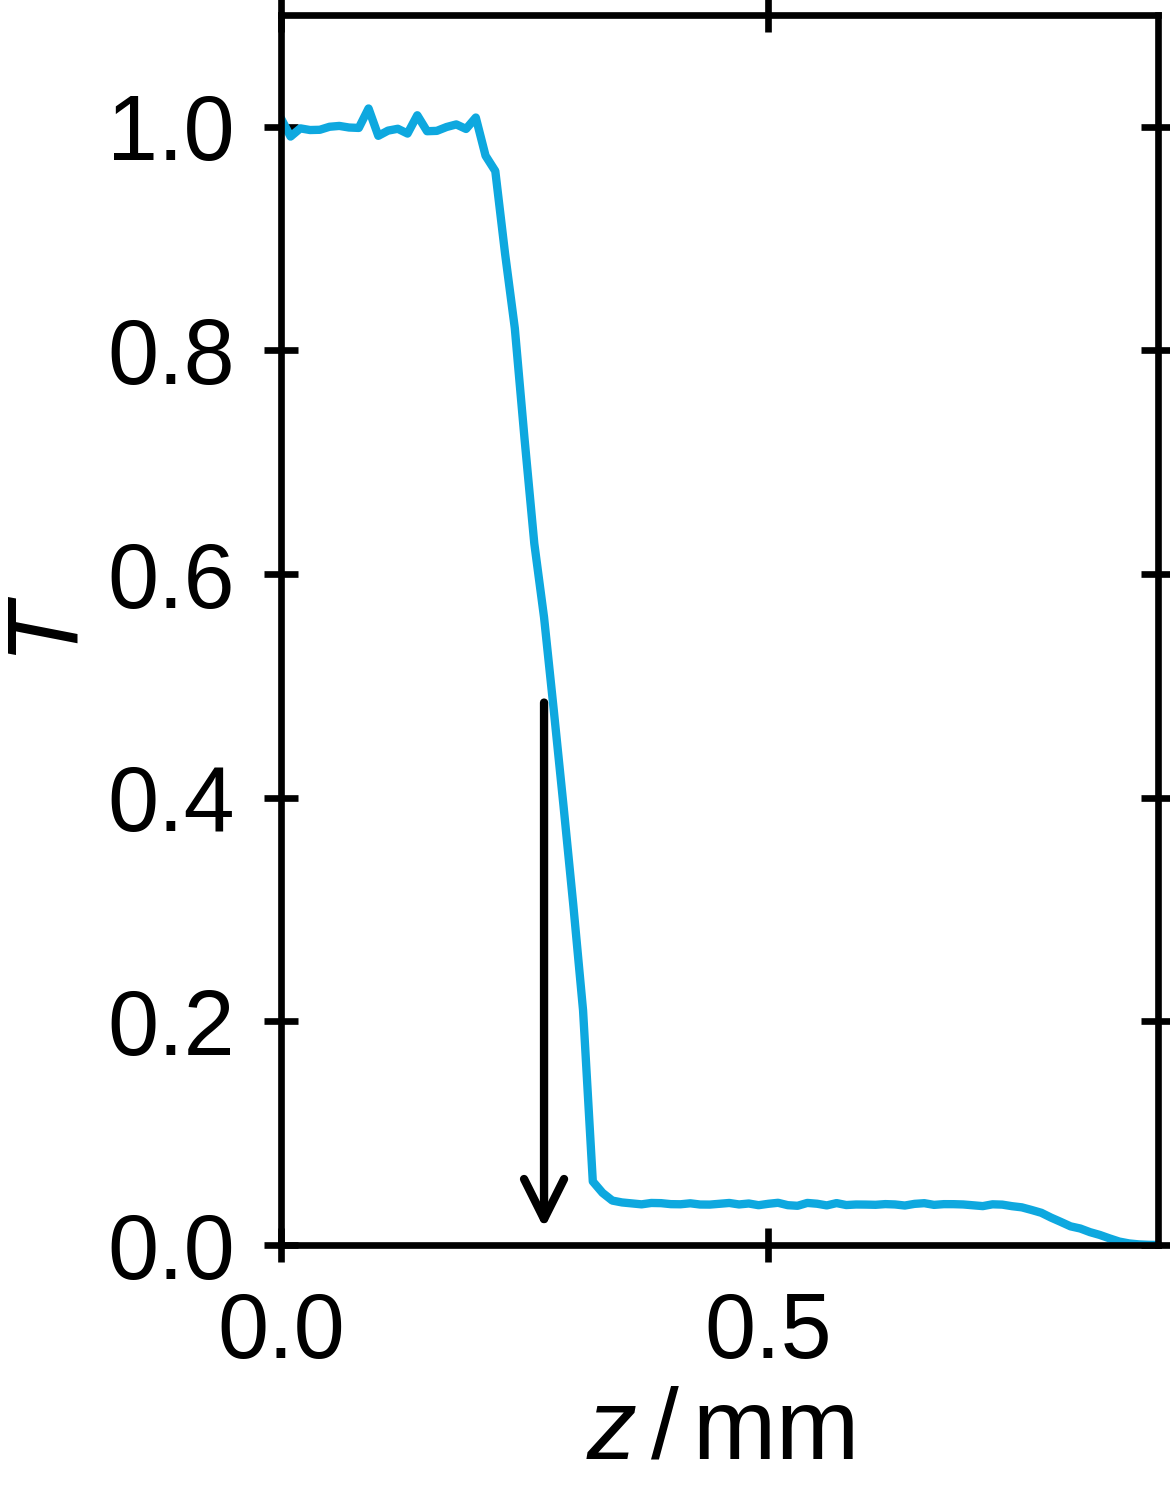
\includegraphics{appendix_methods_XRR_zScan}
      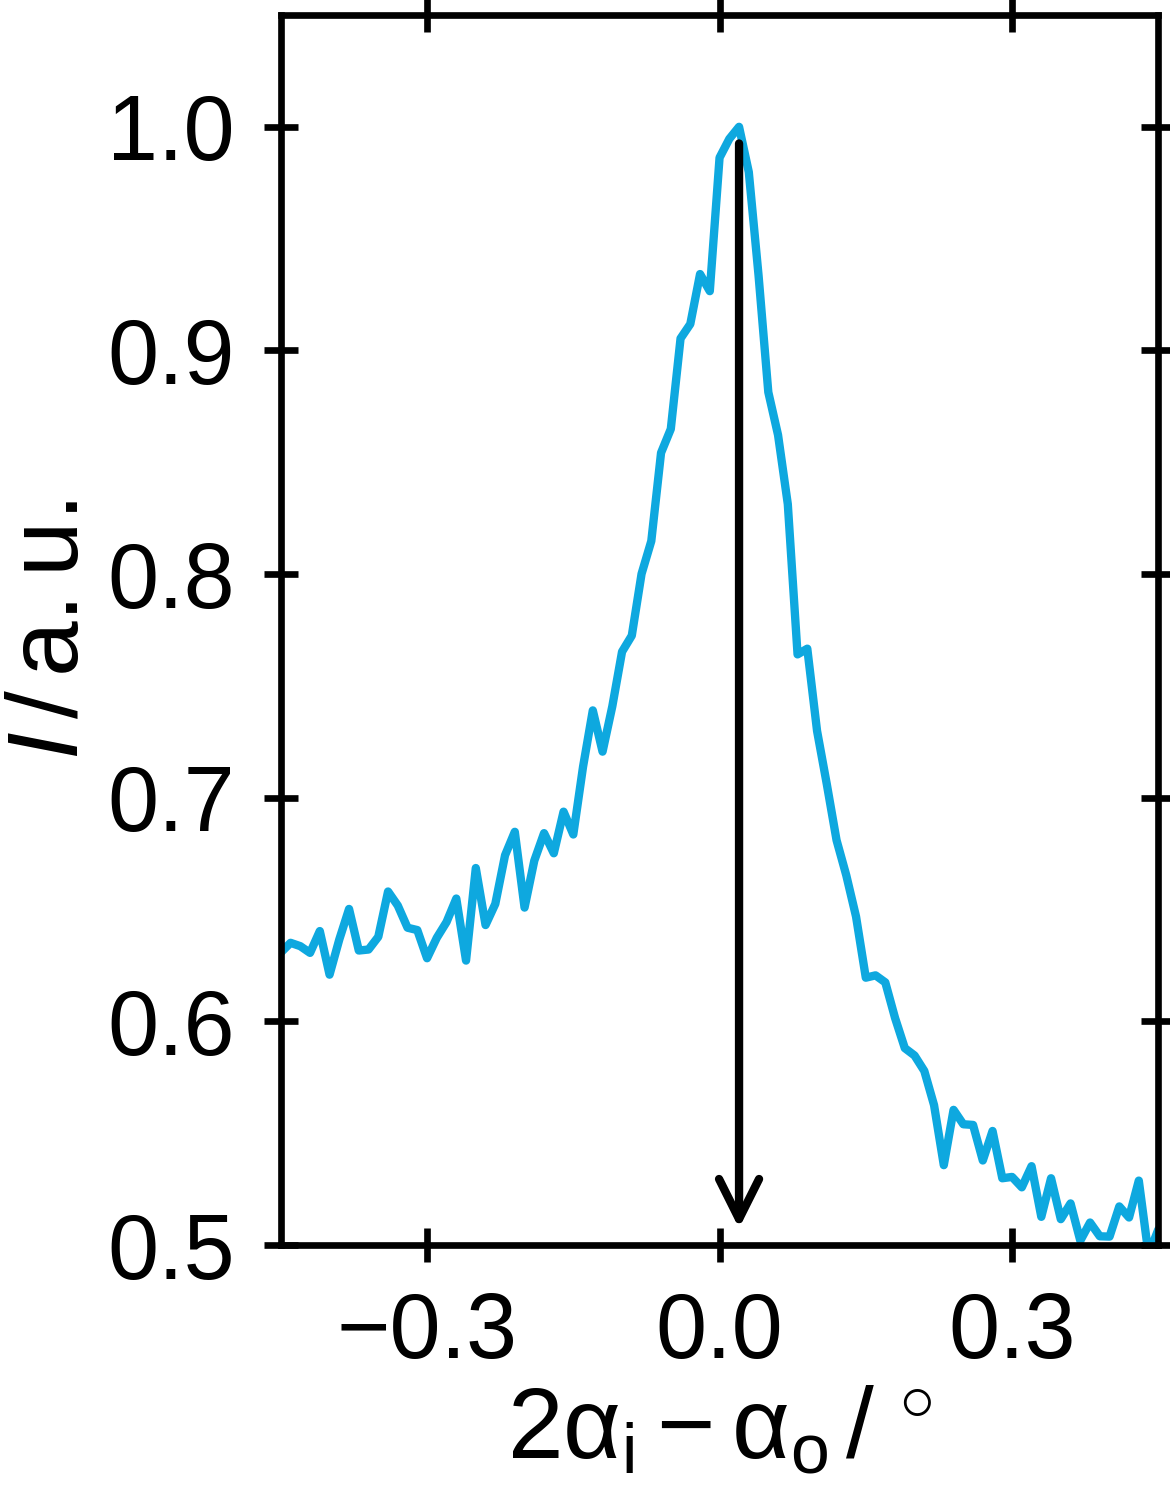
\includegraphics{appendix_methods_XRR_rockingCurve_zero}
      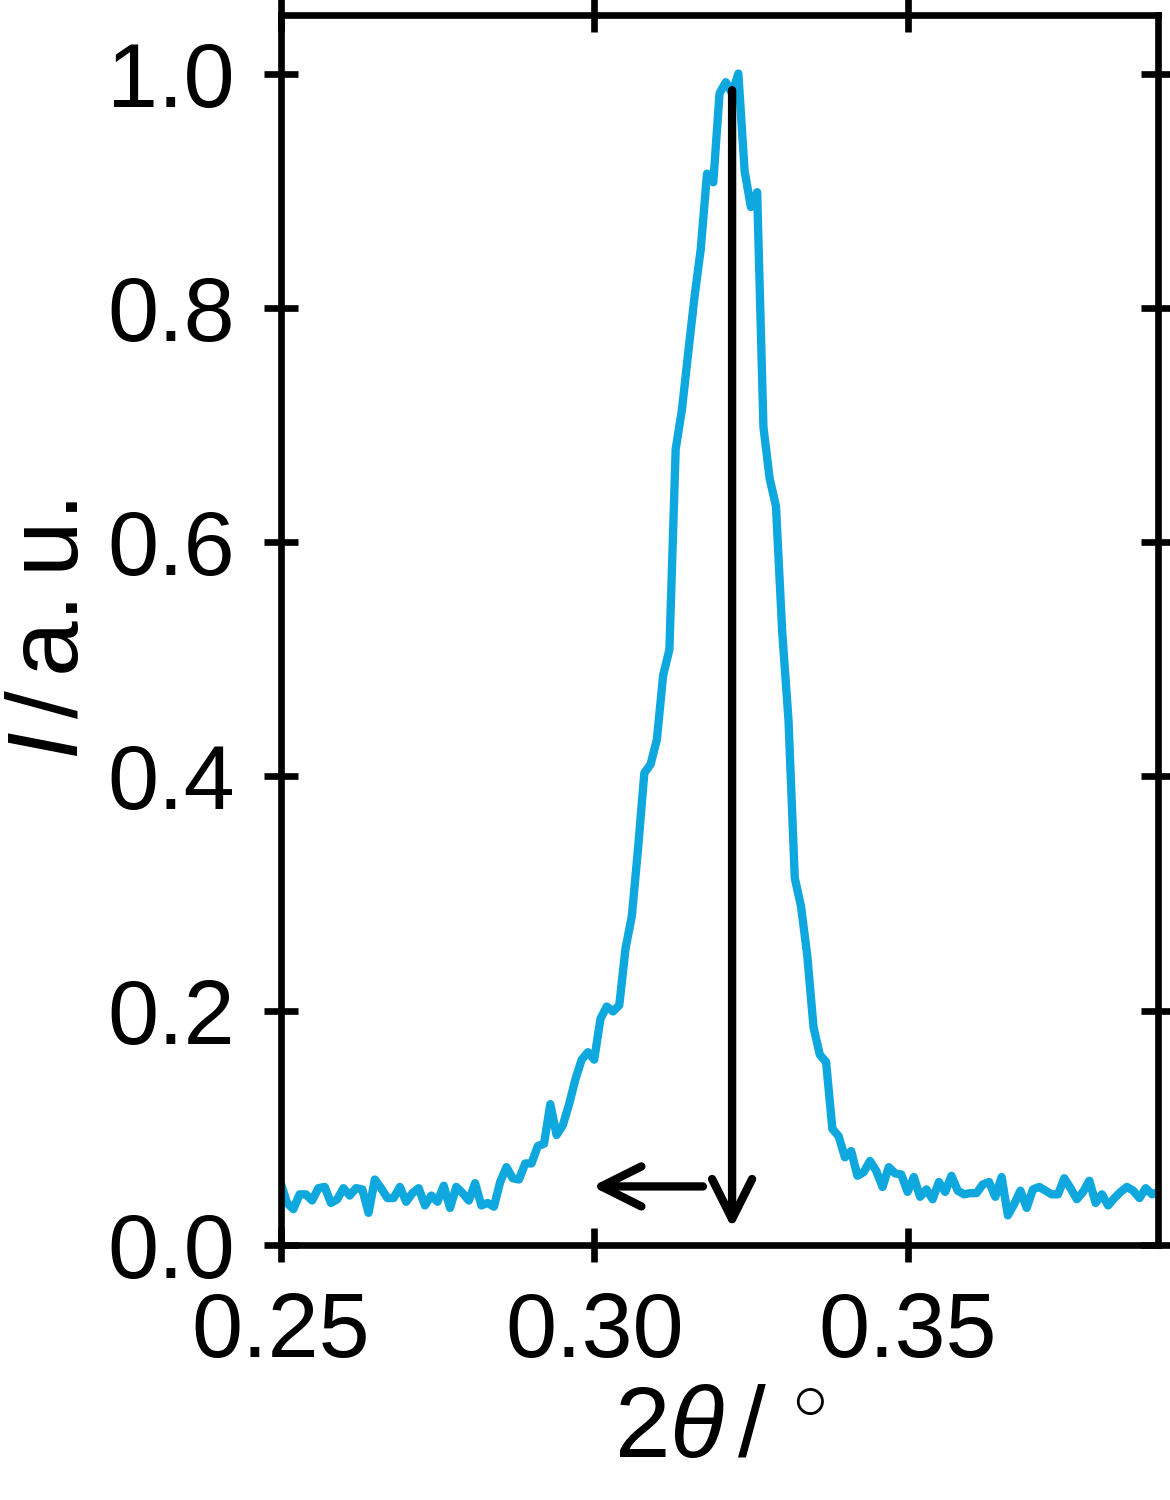
\includegraphics{appendix_methods_XRR_rockingCurve_reflection}
      \caption{\label{fig:appendix:methods:xrr:alignment}.}
    \end{figure}

    X-ray reflectometry can typically measured on a commercial laboratory instrument such as the Bruker D8 of the \textsc{Forschungszentrum J\"ulich} \refapp{app:additionalExperimentalTechniques:xrr}, which was used in this thesis.
    In a typical experiment, the sample is placed in the center between a X-ray source and a detector, which both can be independently moved from one another at a fixed distance with the angles $\alpha_i$ for the source and $\alpha_o$ for the detector.
    The sample stage is a flat surface that can be moved vertically.
    To center the sample and to have it oriented with respect to the source and detector three alignment procedures are performed.
    By performing a scan of the transmitted X-rays with respect to the vertically moving sample at both $0^\circ$ angle for source and detector, the sample is centered by choosing the position at the value where the X-ray beam is halved as depicted in the left plot of \reffig{fig:appendix:methods:xrr:alignment}.
    An absorption triangle is measured, by setting $\alpha_i$ and $\alpha_o$ to the presumably zero values first and performing a rocking curve then, where $\alpha_i + \alpha_o \eq 0^\circ$ is fixed (\reffig{fig:appendix:methods:xrr:alignment}, center).
    The positions at the peak value are set to zero for $\alpha_i$ and $\alpha_o$.
    Then to improve this alignment, $\alpha_i$ and $\alpha_f$ is set to some angle still close to the critical angle such as $0.3^\circ$ and another rocking scan is performed where again $\alpha_i + \alpha_o$ is fixed.
    As visible in the right plot of \reffig{fig:appendix:methods:xrr:alignment}, a peak is visible from which both $\alpha_i$ and $\alpha_o$ can then be calibrated by the peak position to the expected angle that was chosen.
    These steps are repeated until no recalibration factors need to be applied anymore and the alignment measurements agree with the expectation.

    \begin{figure}[tb]
      \centering
      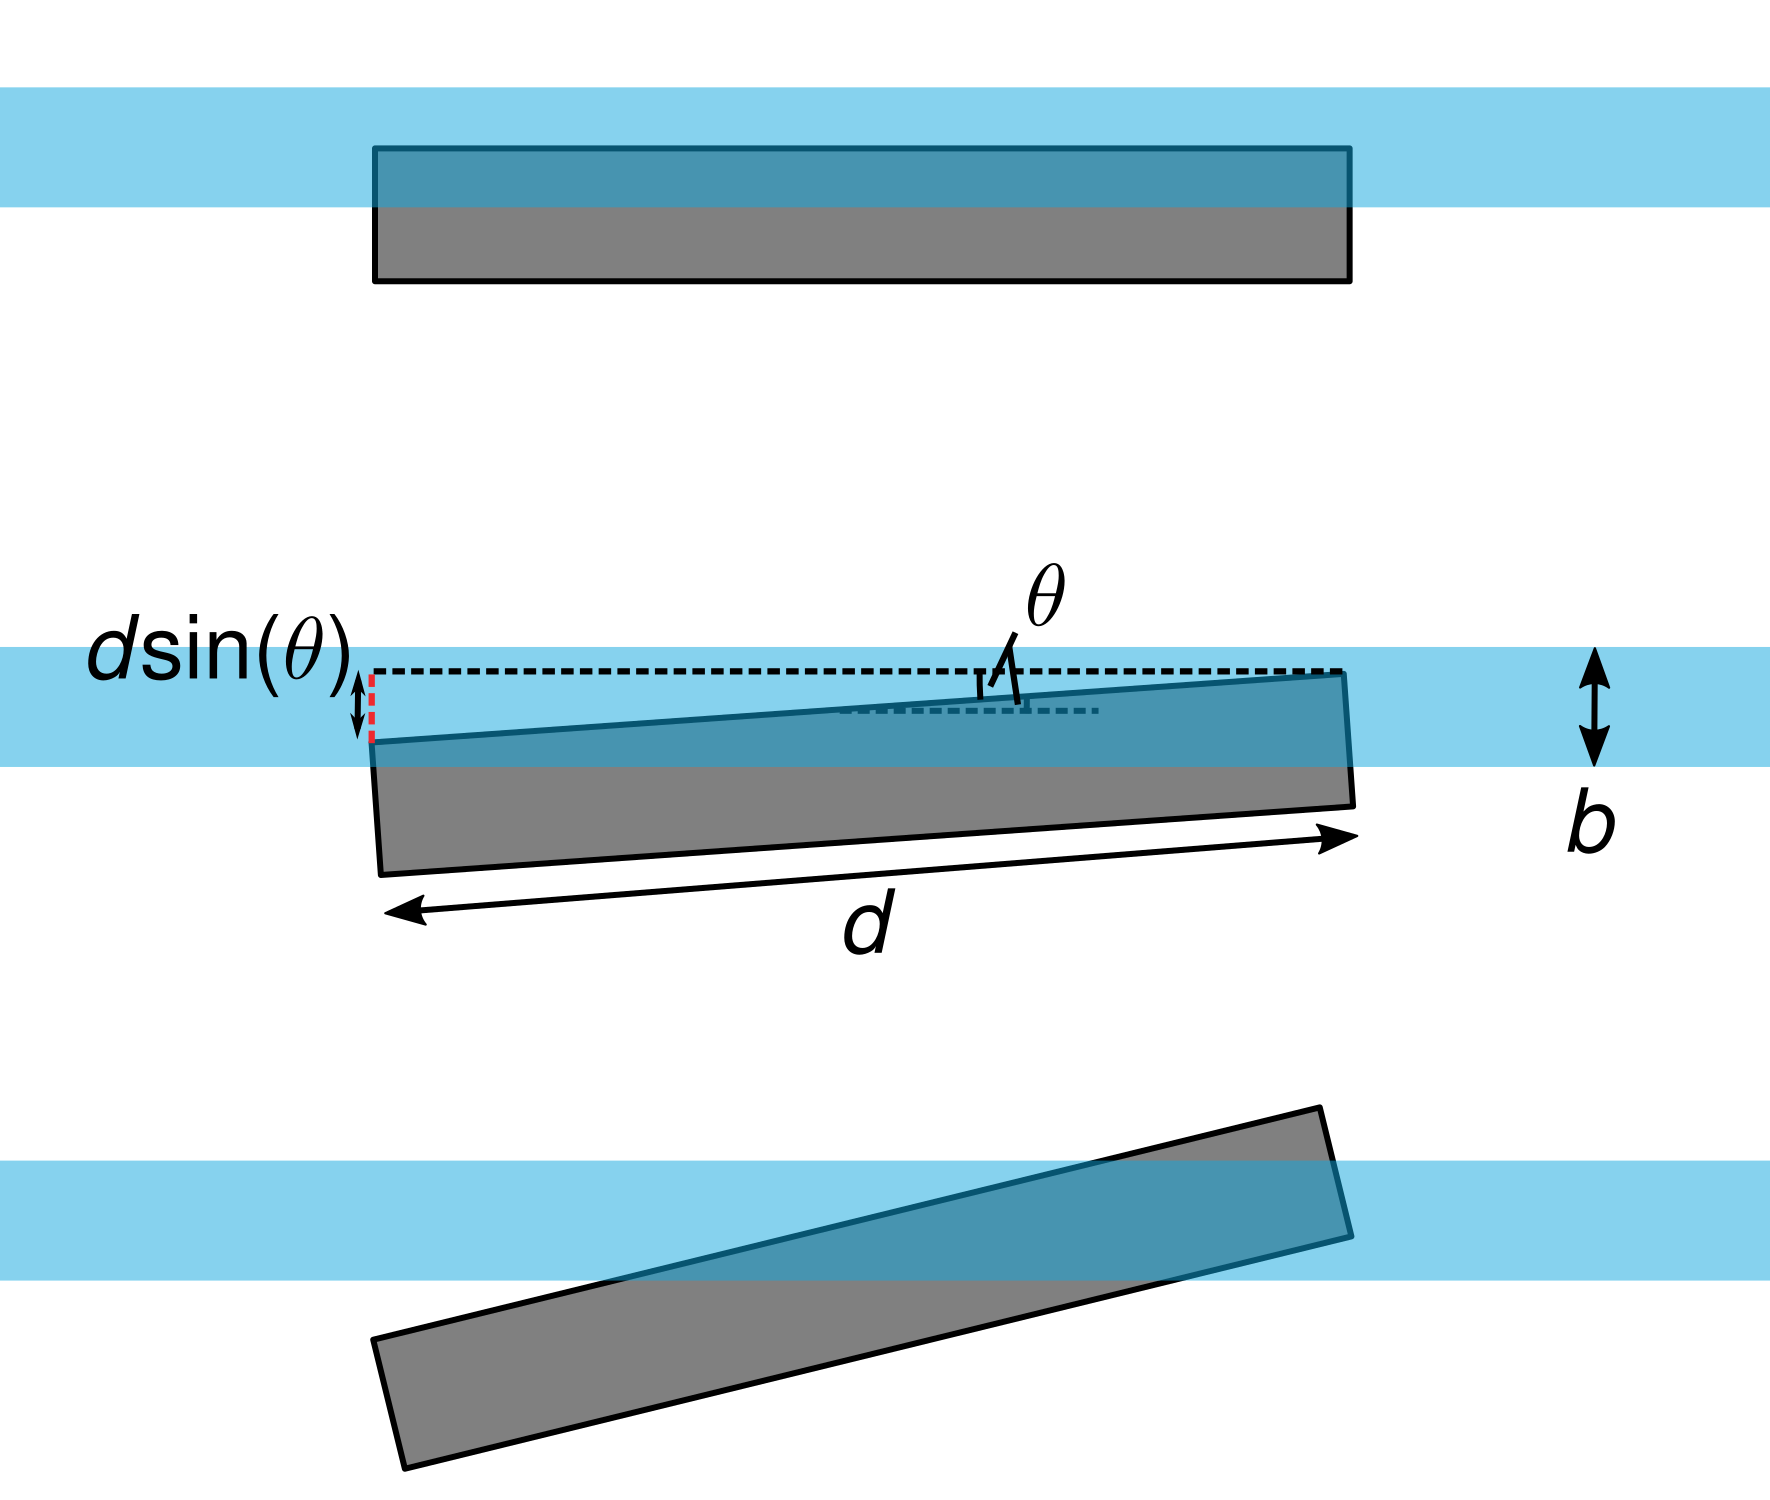
\includegraphics{appendix_methods_XRR_footprint}
      \caption{\label{fig:appendix:methods:xrr:footprint}Depiction of the footprint from the beam on the sample. At small angles }
    \end{figure}

    In an experiment, the XRR profile is then obtained by moving source and detector and counting the scattered X-rays under specular condition $\alpha_i \eq \alpha_o \eq \theta$ with respect to the incident angle.
    As typically the footprint of the beam on the sample is initially larger than the sample size, no plateau is measured for small angles as expected but the intensity increases until the complete beam hits the sample as shown in \reffig{fig:appendix:methods:xrr:footprint}.
    The effect of the footprint can be corrected by knowledge of the beam size and the sample dimension along the beam direction \cite{Gibaud_1993_Theco}.
    For a beam with a normalized intensity profile $g(x)$ profile and a sample size of $d$, the correction is performed by
    \begin{align}
      I_\mathrm{footpr. corr.}(\theta) \eq I_\mathrm{meas.}(\theta) \Biggl( \int_{-\tfrac{1}{2}d \sin(\theta)}^{\tfrac{1}{2}d \sin(\theta)} g(x) \dint x \Biggr)^{-1},
    \end{align}
    where the coordinate axis is set such that zero is in the center of the beam.
    For a equidistribution of the intensity in the beam
    \begin{align}
      g_\mathrm{equidist.}(x) \eq \begin{cases}
        \frac{1}{b}& \mathrm{for\,}-\frac{b}{2} < x < \frac{b}{2},\\
        0&\mathrm{else},
      \end{cases}
    \end{align}
    the footprint correction is given by
    \begin{align}
      I_\mathrm{footpr. corr.}^\mathrm{equidist.}(\theta) \eq I_\mathrm{meas.}(\theta) \Biggl( \frac{b}{d \sin(\theta)}\Biggr)^{-1},\hspace{2cm}\mathrm{for\,}d\sin(\theta)<b ,
    \end{align}
    which is approximately linear for small angles.
    For a Gaussian beam profile, the correction is given in terms of the error function $\mathrm{erf}(x)$
    \begin{align}
      I_\mathrm{footpr. corr.}^\mathrm{Gaussian}(\theta) \eq I(\theta) \Biggl( \mathrm{erf}\biggl( \frac{d \sin(\theta)}{\sqrt{2}b} \biggr) \Biggr)^{-1}.
    \end{align}
    In this case the width of the Gaussian is defined as $b \eq 2 \sigma$, which includes $\approx 68 \%$ of the intensity.

    The data is then finally scaled by calculating the mean value of an area on the plateau and setting it to one.
    The reflectivity curve is then discussed in terms of models of vertical scattering length density profiles, which reproduce the characteristics of the data.
    Typically, a range of $\theta \eq 0^\circ \ldots 3^\circ$ is measured in this thesis in a step size of $0.005^\circ$, which corresponds to a $q$ range of $0 \ldots 2 \unit{nm^{-1}}$ and $\Delta q \approx 0.007 \unit{nm^{-1}}$.
    In this manner length scales up to $\approx 900 \unit{nm}$ can ideally be characterized with a resolution of $3 \unit{nm}$.
\end{document}